\chapter{Implementation}
\label{chap:implementation}

DortDB is a collection of TypeScript libraries. Its source code is available as an appendix to this thesis, as well as online at \href{https://github.com/filipjezek/dortdb}{https://github.com/filipjezek/dortdb}. All the libraries are part of a single monorepository managed with Nx\footnote{\url{https://nx.dev/}}. The \texttt{@dortdb/core} is the main library containing the core of the framework. There is a separate library for each of the currently implemented languages (\texttt{@dortb/lang-cypher}, \texttt{@dortdb/lang-sql}, and \texttt{@dortdb/lang-xquery}). Additionally, there are packages for the GUI and benchmarks (\texttt{@dortdb/showcase} and \texttt{@dortdb/benchmarks}). Finally, \texttt{@dortdb/dataloaders} contains utilities for importing data from various formats.

\begin{figure}[htpb]
    \centering
    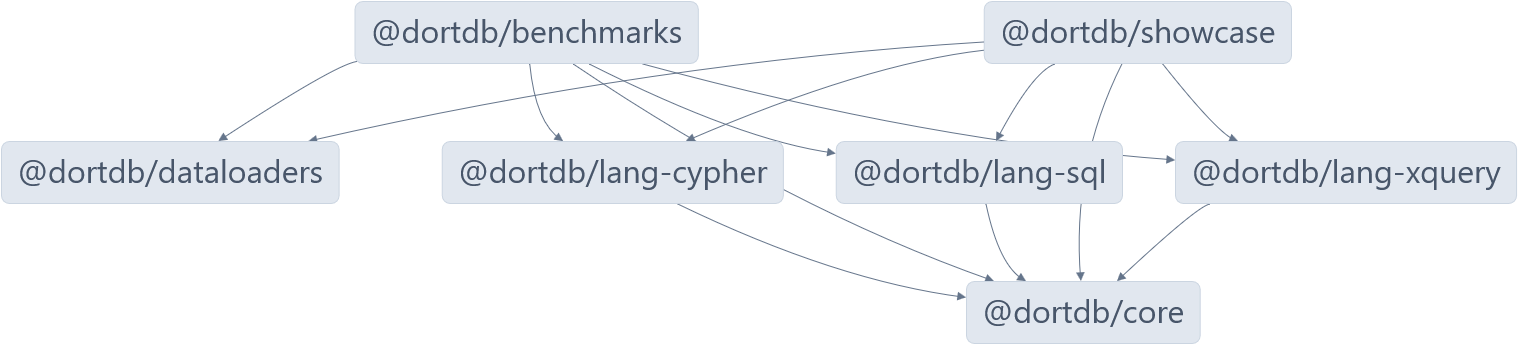
\includegraphics[width=\textwidth]{img/packages-graph.png}
    \caption{Dependency graph of the monorepository.}
\end{figure}

\section{Core library}

The core library serves as a common framework for registering data sources, querying, and optimization. The individual languages are responsible for converting a text query into a logical plan. The plan operator tree implements an extended version of the visitor design pattern\cite{johnson1995design}. In order for each language to be able to expand the plan algebra with its own operators, or to customize the behavior defined for a common operator, the design pattern is modified to take into account the language that instantiates each plan operator, as seen in Figure \ref{fig:visitor-pattern}. The \texttt{accept} method accepts a dictionary of visitors instead of a single visitor. The core library provides a default implementation of a visitor for each phase of the query process. The individual languages may specify their own implementations, usually by extending the original class. The \texttt{accept} and \texttt{visit} methods also optionally take a second argument, which may be necessary to propagate information during the downward pass of the plan tree, for example, the existing context during plan execution.

\begin{listing}[ht!]
    \begin{minted}[fontsize=\small]{ts}
export interface PlanOperator {
  lang: Lowercase<string>;

  accept<Ret, Arg>(
    visitors: Record<string, PlanVisitor<Ret, Arg>>,
    arg?: Arg,
  ): Ret;

  // ...
}
    
export interface PlanVisitor<Ret, Arg = never> {
  visitRecursion(operator: Recursion, arg?: Arg): Ret;
  visitItemSource(operator: ItemSource, arg?: Arg): Ret;
  visitProjection(operator: Projection, arg?: Arg): Ret;
  // ...
}

export class ItemSource implements PlanOperator {
  constructor(
    public lang: Lowercase<string>,
    public name: ASTIdentifier | Aliased<ASTIdentifier>,
  ) {}

  accept<Ret, Arg>(
    visitors: Record<string, PlanVisitor<Ret, Arg>>,
    arg?: Arg,
  ): Ret {
    return visitors[this.lang].visitItemSource(this, arg);
  }

  // ...
}
    \end{minted}
    \caption{The extended visitor pattern used in the logical plan.}
    \label{fig:visitor-pattern}
\end{listing}

\subsection{Language manager}

Each language can define its own visitors, callables, or aggregates. Callables and aggregates may also be provided as an extension, not scoped to any specific language. For example, a datetime extension might define operators and functions for manipulating datetime values. The \texttt{LanguageManager} class then handles instantiating of visitor dictionaries or finding an aggregate or callable by name.

\section{Query process}

The rest of the library's key components will be outlined in the order they appear during query execution. Different languages may handle some steps differently. The key deviations will be noted when appropriate.

\subsection{Lexer and parser}

First of all, the text query needs to be parsed into an \textit{abstract syntax tree (AST)}. In order to do this, \textit{parser generators} are used. Modern projects use solutions such as \texttt{ANTLR}\footnote{\url{https://www.antlr-ng.org/}}. We have used 
\texttt{ts-jison}\footnote{\url{https://github.com/ericprud/ts-jison}} instead, which is based on \texttt{GNU Bison}\footnote{\url{https://www.gnu.org/software/bison/}}. \texttt{Bison} employs an older approach less compatible with modern software engineering practices. The resulting parser and its runtime are, however, significantly smaller (approximately 10 times).

The parser is generated from a formal grammar file. \texttt{ts-jison} in fact generates two components. The \textit{lexer} handles the lexical analysis, converting the text query into tokens such as a specific keyword or a string. The parser then combines the tokens into grammar constructs like a function call or a \texttt{SELECT} statement. The resulting AST nodes implement the visitor pattern, similarly to the logical plan.

\subsection{Plan builder}

The AST is converted into a logical plan using a \texttt{PlanBuilder} visitor. It is possible to apply some optimizations while creating the plan, but the resulting plan is mostly a literal representation of the original query. Intermediary operators are converted into \texttt{calculations} right at this stage, in a process more closely described in section \ref{sec:calc-building}. The SQL language creates the plan in two passes, for reasons detailed in section \ref{subsec:sql-schema-data-sources}. The plan builder is provided the current context in order to determine which attributes are variables or columns, etc, and which should be considered data sources. Some languages (like SQL) do not know the full context when building plans for nested language subqueries. The context, therefore, also includes information on data sources whose schema is being inferred. The plan builder should, in addition to the plan, create a set of newly identified identifiers. See Program \ref{fig:plan-builder-outer-ctx} for an example.

\begin{listing}[!ht]
\begin{minted}{sql}
SELECT attr1 FROM t1
WHERE EXISTS (
  LANG xquery
\end{minted}
\nestedMintedVspace
\begin{minted}[style=manni]{xquery}
  $Invoices//[OrderId = $t1:attr2]
\end{minted}
\nestedMintedVspace
\begin{minted}{sql}
)
\end{minted}
\caption{The plan builder for XQuery receives context with \texttt{t1.attr1} and with \texttt{t1} set as a data source with not yet identified schema. It then correctly interprets \texttt{\$t1:attr2} as a variable and \texttt{\$Invoices} as a data source. The SQL plan builder then receives back information on \texttt{t1.attr2}.}
\label{fig:plan-builder-outer-ctx}
\end{listing}

\subsection{Optimizer et al.}

The optimizer itself and its rules have their own section elsewhere, see \ref{sec:optimizer}. They make use of multiple other plan visitors.

\begin{description}
    \item[\texttt{EqualityChecker}] A deep equality checker. It is possible to check equality of plan operator trees regardless of their language, or with specific renamings applied. This is helpful, for example, when checking possibly indexable expressions in a \texttt{join} operator, whose input \texttt{tupleSources} are renamed with a \texttt{projection}.
    \item[\texttt{AttributeRenamer}] This visitor renames attributes in an operator tree. Necessary when, e.g., pushing down \texttt{selections} below \texttt{projections}.
    \item[\texttt{AttributeRenameChecker}] It is not always possible to rename attributes without changing the meaning of a query. This visitor verifies that a specific renaming can be done. See figure \ref{fig:cannot-rename} for an example.
    \item[\texttt{TransitiveDependencies}] This visitor extracts dependencies of an operator tree, helping to identify correlated subqueries. As an example, \mint{sql}/SELECT foo.x FROM foo WHERE bar.y > foo.z/ depends on external attribute \texttt{bar.y}. Used in many rules, among others, in selection pushdown or projection merging.
\end{description}

\subsection{Variable mapper}

Attributes used in queries and their plans can generally have multiple components, for example \mintinline{text}{schema.table.column} or \mintinline{xquery}{$qualified:variable}. During query planning and optimization, the attributes are represented as lists of tokens. Sets or maps of attributes are then represented using tries made of nested hash tables. This is fine during planning, but if that were the case during execution and tuples were represented using the same tries, attribute lookups would become prohibitively expensive. In order to optimize this, the \texttt{VariableMapper} visitor renames all attributes as a single number. During execution, tuples are then represented using simple arrays. The numeric attributes are reused when possible to keep the array sizes minimal.

\subsection{Data adapters}

Different data models and different languages may make different assumptions about how the data is stored or represented. In order to decouple logical plans from the data, languages can be configured with data adapters. Data adapters specify how data sources should be accessed. For example, the default XQuery data adapter allows \texttt{treeStep} operators to traverse XML elements. It may, however, be desirable to use XQuery to query JSON data instead. Cypher queries target graphs, which can also be stored in multiple ways. Nodes might be JavaScript objects, and edges might be their properties. The graph might also be stored as a collection of relations, one for each node or edge type. The default Cypher data adapter uses Graphology\cite{guillaume_plique_2025_14835805} as the data backend. The SQL data adapter can be used to override how SQL accesses attributes in relations.

\begin{listing}[ht!]
    \begin{minted}[fontsize=\small]{ts}
export interface XQueryDataAdapter<NodeType = any> {
  isNode(node: unknown): node is NodeType;
  treeStep(test: ASTItemType, axis: AxisType): (node: NodeType) => NodeType[];
  createElement(ns: string, qname: string, content: unknown[]): NodeType;
  createAttribute(ns: string, qname: string, content: string): NodeType;
  createComment(content: string): NodeType;
  createDocument(ns: string, qname: string, content: unknown[]): NodeType;
  createNS(name: string, content: string): NodeType;
  createText(content: string): NodeType;
  createProcInstr(name: string, content: string): NodeType;
  addAttribute(el: NodeType, attr: NodeType): void;
  lookupPrefix(el: NodeType, ns: string): string;
  lookupNSUri(el: NodeType, prefix: string): string;
  atomize(value: unknown): unknown;
}
    \end{minted}
    \caption{The XQuery data adapter interface}
\end{listing}

\subsection{Executor}

Finally, the logical plan is executed. Unlike other visitors, the \texttt{Executor} provided by the core library is abstract and not immediately usable. As was touched upon in previous sections, tuple representations during execution will be different from the actual tuples available in the source data. Each language should therefore extend the \texttt{Executor} and provide its own implementation of the \texttt{visitTupleSource} method.

The default executor implementation makes heavy use of iterators. This comes with a performance impact for smaller datasets, but for larger amounts of data, the difference becomes negligible. This is compensated by memory efficiency. Unless an operator needs to load all of its inputs fully into memory (for example, if it is \texttt{orderBy} or \texttt{groupBy}), the operator produces values on demand lazily. The default executor implementation is fully synchronous and does not support user-defined functions that return promises (e.g., a \texttt{tupleFnSource} which would load a remote JSON document). The visitor pattern, however, makes it easy to make another executor implementation that would add such functionality.

After the query results are produced, tuple values must be serialized into a suitable representation. To this end, each language may specify a serializer function. The default serializer function joins attribute parts with periods and creates a JavaScript object for each tuple.